%%%%%%%%%%%%%%%%%%%%%%%%%%%%%%%%%%%%%%%%%
% Programming/Coding Assignment
% LaTeX Template
%
% This template has been downloaded from:
% http://www.latextemplates.com
%
% Original author:
% Ted Pavlic (http://www.tedpavlic.com)
%
% Note:
% The \lipsum[#] commands throughout this template generate dummy text
% to fill the template out. These commands should all be removed when 
% writing assignment content.
%
% This template uses a Perl script as an example snippet of code, most other
% languages are also usable. Configure them in the "CODE INCLUSION 
% CONFIGURATION" section.
%
%%%%%%%%%%%%%%%%%%%%%%%%%%%%%%%%%%%%%%%%%

%----------------------------------------------------------------------------------------
%	PACKAGES AND OTHER DOCUMENT CONFIGURATIONS
%----------------------------------------------------------------------------------------

\documentclass{article}

\usepackage{fancyhdr} % Required for custom headers
\usepackage{lastpage} % Required to determine the last page for the footer
\usepackage{extramarks} % Required for headers and footers
\usepackage[usenames,dvipsnames]{color} % Required for custom colors
\usepackage{graphicx} % Required to insert images
\usepackage{subcaption}
\usepackage{listings} % Required for insertion of code
\usepackage{courier} % Required for the courier font
\usepackage{lipsum} % Used for inserting dummy 'Lorem ipsum' text into the template

% Margins
\topmargin=-0.45in
\evensidemargin=0in
\oddsidemargin=0in
\textwidth=6.5in
\textheight=9.0in
\headsep=0.25in

\linespread{1.1} % Line spacing

% Set up the header and footer
\pagestyle{fancy}
\lhead{\hmwkAuthorName} % Top left header
\chead{\hmwkClass\ (\hmwkClassTime): \hmwkTitle} % Top center head
%\rhead{\firstxmark} % Top right header
\lfoot{\lastxmark} % Bottom left footer
\cfoot{} % Bottom center footer
\rfoot{Page\ \thepage\ of\ \protect\pageref{LastPage}} % Bottom right footer
\renewcommand\headrulewidth{0.4pt} % Size of the header rule
\renewcommand\footrulewidth{0.4pt} % Size of the footer rule

\setlength\parindent{0pt} % Removes all indentation from paragraphs

%----------------------------------------------------------------------------------------
%	CODE INCLUSION CONFIGURATION
%----------------------------------------------------------------------------------------

\definecolor{MyDarkGreen}{rgb}{0.0,0.4,0.0} % This is the color used for comments
\lstloadlanguages{Perl} % Load Perl syntax for listings, for a list of other languages supported see: ftp://ftp.tex.ac.uk/tex-archive/macros/latex/contrib/listings/listings.pdf
\lstset{language=Perl, % Use Perl in this example
        frame=single, % Single frame around code
        basicstyle=\small\ttfamily, % Use small true type font
        keywordstyle=[1]\color{Blue}\bf, % Perl functions bold and blue
        keywordstyle=[2]\color{Purple}, % Perl function arguments purple
        keywordstyle=[3]\color{Blue}\underbar, % Custom functions underlined and blue
        identifierstyle=, % Nothing special about identifiers                                         
        commentstyle=\usefont{T1}{pcr}{m}{sl}\color{MyDarkGreen}\small, % Comments small dark green courier font
        stringstyle=\color{Purple}, % Strings are purple
        showstringspaces=false, % Don't put marks in string spaces
        tabsize=5, % 5 spaces per tab
        %
        % Put standard Perl functions not included in the default language here
        morekeywords={rand},
        %
        % Put Perl function parameters here
        morekeywords=[2]{on, off, interp},
        %
        % Put user defined functions here
        morekeywords=[3]{test},
       	%
        morecomment=[l][\color{Blue}]{...}, % Line continuation (...) like blue comment
        numbers=left, % Line numbers on left
        firstnumber=1, % Line numbers start with line 1
        numberstyle=\tiny\color{Blue}, % Line numbers are blue and small
        stepnumber=5 % Line numbers go in steps of 5
}

% Creates a new command to include a perl script, the first parameter is the filename of the script (without .pl), the second parameter is the caption
\newcommand{\perlscript}[2]{
\begin{itemize}
\item[]\lstinputlisting[caption=#2,label=#1]{#1.pl}
\end{itemize}
}

%----------------------------------------------------------------------------------------
%	DOCUMENT STRUCTURE COMMANDS
%	Skip this unless you know what you're doing
%----------------------------------------------------------------------------------------

% Header and footer for when a page split occurs within a problem environment
\newcommand{\enterProblemHeader}[1]{
%\nobreak\extramarks{#1}{#1 continued on next page\ldots}\nobreak
%\nobreak\extramarks{#1 (continued)}{#1 continued on next page\ldots}\nobreak
}

% Header and footer for when a page split occurs between problem environments
\newcommand{\exitProblemHeader}[1]{
%\nobreak\extramarks{#1 (continued)}{#1 continued on next page\ldots}\nobreak
%\nobreak\extramarks{#1}{}\nobreak
}

\setcounter{secnumdepth}{0} % Removes default section numbers
\newcounter{homeworkProblemCounter} % Creates a counter to keep track of the number of problems
\setcounter{homeworkProblemCounter}{0}

\newcommand{\homeworkProblemName}{}
\newenvironment{homeworkProblem}[1][Part \arabic{homeworkProblemCounter}]{ % Makes a new environment called homeworkProblem which takes 1 argument (custom name) but the default is "Problem #"
\stepcounter{homeworkProblemCounter} % Increase counter for number of problems
\renewcommand{\homeworkProblemName}{#1} % Assign \homeworkProblemName the name of the problem
\section{\homeworkProblemName} % Make a section in the document with the custom problem count
\enterProblemHeader{\homeworkProblemName} % Header and footer within the environment
}{
\exitProblemHeader{\homeworkProblemName} % Header and footer after the environment
}

\newcommand{\problemAnswer}[1]{ % Defines the problem answer command with the content as the only argument
\noindent\framebox[\columnwidth][c]{\begin{minipage}{0.98\columnwidth}#1\end{minipage}} % Makes the box around the problem answer and puts the content inside
}

\newcommand{\homeworkSectionName}{}
\newenvironment{homeworkSection}[1]{ % New environment for sections within homework problems, takes 1 argument - the name of the section
\renewcommand{\homeworkSectionName}{#1} % Assign \homeworkSectionName to the name of the section from the environment argument
\subsection{\homeworkSectionName} % Make a subsection with the custom name of the subsection
\enterProblemHeader{\homeworkProblemName\ [\homeworkSectionName]} % Header and footer within the environment
}{
\enterProblemHeader{\homeworkProblemName} % Header and footer after the environment
}

%----------------------------------------------------------------------------------------
%	NAME AND CLASS SECTION
%----------------------------------------------------------------------------------------

\newcommand{\hmwkTitle}{Assignment\ \#$1$(run on macOS10.13.1)} % Assignment title
\newcommand{\hmwkDueDate}{Monday,\ January\ 29,\ 2018} % Due date
\newcommand{\hmwkClass}{CSC411} % Course/class
\newcommand{\hmwkClassTime}{L0101} % Class/lecture time
\newcommand{\hmwkAuthorName}{Yufeng Li} % Your name

%----------------------------------------------------------------------------------------
%	TITLE PAGE
%----------------------------------------------------------------------------------------

\title{
\vspace{2in}
\textmd{\textbf{\hmwkClass:\ \hmwkTitle}}\\
\normalsize\vspace{0.1in}\small{Due\ on\ \hmwkDueDate}\\
\vspace{0.1in}
\vspace{3in}
}

\author{\textbf{\hmwkAuthorName}}
%\date{} % Insert date here if you want it to appear below your name

%----------------------------------------------------------------------------------------

\begin{document}

\maketitle
\clearpage
%----------------------------------------------------------------------------------------
%	PROBLEM 1
%----------------------------------------------------------------------------------------

% To have just one problem per page, simply put a \clearpage after each problem

\begin{homeworkProblem}
The number of pictures I obtained are as follows:
\begin{verbatim}
uncropped:             
vartan 195
radcliffe 214
gilpin 189
drescher 239
hader 278
ferrera 246
chenoweth 257
bracco 216
butler 198
baldwin 266
carell 264
harmon 239

cropped:
vartan 189
radcliffe 196
gilpin 171
drescher 221
hader 236
ferrera 233
chenoweth 228
bracco 184
butler 184
baldwin 232
carell 236
harmon 195
\end{verbatim}
\clearpage
On the lefthand side are the uncropped images(resized to better compare,the original size is bigger),on the righthand side are the cropped and been switched to greyscale.(32*32)

\begin{figure*}[!ht]
\begin{subfigure}{.35\textwidth}
  \centering
  \includegraphics[width=.35\linewidth]{baldwin0un.jpg}
  \caption{}
  \label{fig:1}
\end{subfigure}%
\begin{subfigure}{.35\textwidth}
  \centering
  \includegraphics[width=.35\linewidth]{baldwin0cr.jpg}
  \caption{}
  \label{fig:2}
\end{subfigure}%
\break
\begin{subfigure}{.35\textwidth}
  \centering
  \includegraphics[width=.35\linewidth]{baldwin13un.jpg}
  \caption{}
  \label{fig:3}
\end{subfigure}%
\begin{subfigure}{.35\textwidth}
  \centering
  \includegraphics[width=.35\linewidth]{baldwin13cr.jpg}
  \caption{}
  \label{fig:4}
\end{subfigure}%
\break
\begin{subfigure}{.35\textwidth}
  \centering
  \includegraphics[width=.35\linewidth]{baldwin20un.jpg}
  \caption{}
  \label{fig:5}
\end{subfigure}%
\begin{subfigure}{.35\textwidth}
  \centering
  \includegraphics[width=.35\linewidth]{baldwin20cr.jpg}
  \caption{}
  \label{fig:6}
\end{subfigure}%
\end{figure*}
Some of the bounding boxes are not accurate thus creating uncertainty to our training process. However, some cropped picture can align with the uncropped counterpart.
\clearpage
On the lefthand side are the uncropped images(resized to better compare,the original size is bigger),on the righthand side are the cropped and been switched to greyscale.(32*32)
\begin{figure*}[!ht]
\begin{subfigure}{.35\textwidth}
  \centering
  \includegraphics[width=.35\linewidth]{bracco34un.jpg}
  \caption{}
  \label{fig:a0noise0.05}
\end{subfigure}%
\begin{subfigure}{.35\textwidth}
  \centering
  \includegraphics[width=.35\linewidth]{bracco34cr.jpg}
  \caption{}
  \label{fig:a0noise0.05reconstruction}
\end{subfigure}%
\break
\begin{subfigure}{.35\textwidth}
  \centering
  \includegraphics[width=.35\linewidth]{butler41un.jpg}
  \caption{}
  \label{fig:a0noise0.05}
\end{subfigure}%
\begin{subfigure}{.35\textwidth}
  \centering
  \includegraphics[width=.35\linewidth]{butler41cr.jpg}
  \caption{}
  \label{fig:a0noise0.05reconstruction}
\end{subfigure}%
\break
\begin{subfigure}{.35\textwidth}
  \centering
  \includegraphics[width=.35\linewidth]{carell95un.jpg}
  \caption{}
  \label{fig:a0noise0.05}
\end{subfigure}%
\begin{subfigure}{.35\textwidth}
  \centering
  \includegraphics[width=.35\linewidth]{carell95cr.jpg}
  \caption{}
  \label{fig:a0noise0.05reconstruction}
\end{subfigure}%
\end{figure*}
\textit{These are the pictures where the bounding boxes are actually accurate thus they can best represent their faces.}

\end{homeworkProblem}
\clearpage
%----------------------------------------------------------------------------------------
%	PROBLEM 2
%----------------------------------------------------------------------------------------

\begin{homeworkProblem}
\noindent \textit{Separating cropped pictures}

The algorithm I used to separate:
\begin{verbatim}
def group():
    files = os.listdir("cropped")
    names_set = {}
    for file in files:
        name = ''.join([i for i in file if not i.isdigit()]).split('.')[0]
        if name not in names_set:
            names_set[name] = [file]
        else:
            names_set[name].append(file)
    training = []
    validating = []
    testing = []
    count = 0
    for name, files in names_set.items():
        for f in files:
            if count < 70:
                training.append(f)
                count += 1
            if 70 <= count < 80:
                validating.append(f)
                count += 1
            if 80 <= count < 90:
                testing.append(f)
                count += 1
        count = 0
    return names_set, training, validating, testing
\end{verbatim}

At first, it reads "cropped" folder and parse each filename to get its actor name. Then I use that name as a key to my names\_set dictionary followed by all its related filenames list. I used this dictionary to generate my training, validating and testing samples. In practice I use indexes of dictionary's 
value (which is the filename list) to access each sample set of a same actor.


\end{homeworkProblem}
\clearpage
%----------------------------------------------------------------------------------------
%	PROBLEM 3
%----------------------------------------------------------------------------------------

\begin{homeworkProblem}
\noindent \textit{Building classifier to distinguish pictures of Baldwin from that of Carell}
\\
The cost function which I want to minimize is the quadratic loss, which is:(x is sample,y is target, theta is theta)
\begin{verbatim}
    sum((y - dot(theta.T, x)) ** 2)
\end{verbatim}
which then have the result of gradient of loss function like this:
\begin{verbatim}
    -2 * sum((y - dot(theta.T, x)) * x, 1)
\end{verbatim}

To make the gradient descend works, I test out some max iterations and alpha first based on the tutorial code given, I've already strip away those result where it gets NaN or runtime warnings to make the graph looks more reasonable.
\clearpage


\begin{figure*}[!ht]
\begin{subfigure}{.35\textwidth}
  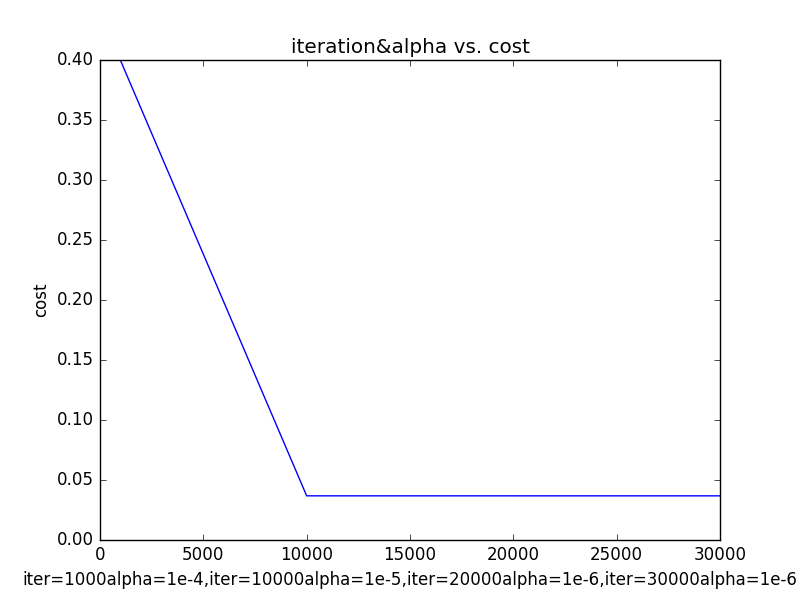
\includegraphics[width=1.5\linewidth]{testiteration.png}
  \caption{Figure 1: Plot of cost function w.r.t. different alpha and max iteration test}
  \label{fig:sfig1}
\end{subfigure}


Figure~\ref{fig:sfig1} demonstrates the effects of decreasing alpha and increase of max iterations.
I use following max iteration and alpha:
maxiter=1000 alpha=1e-4,
maxiter=10000 alpha=1e-5,
maxiter=20000 alpha=1e-6,
maxiter=30000 alpha=1e-6.
As we can see here there's a noticeable decrease in cost when max iteration increase and alpha decreases. The reason why I pick max iteration=30000 and alpha=1e-6 because it produce less error in coding later.



\begin{subfigure}{.35\textwidth}
  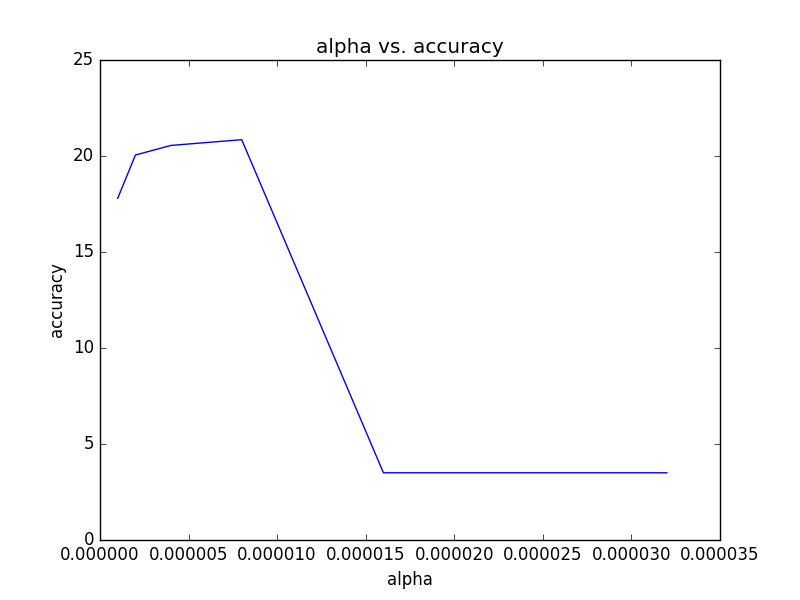
\includegraphics[width=1.5\linewidth]{testalpha.png}
  \caption{Figure 2: Plot of accuracy rate w.r.t. different alpha and fixed max iteration=30000}
  \label{fig:sfig2}
\end{subfigure}

Figure~\ref{fig:sfig2} demonstrates the effects of decreasing alpha and accuracy varies. This is tested on training set of both actors.
As we can see here there's a best range of alphas, I expected that range to have a fluctuated accuracy rate, however for the sake of efficiency i only picked 6 points otherwise it takes too much time to generate. There's a trade off of alpha which is between efficiency and accuracy.

\end{figure*}
\clearpage
\noindent \textit{The result}
\\
The loss using thetas from running training set and validating set is as follows:
\begin{verbatim}
    Loss for training:  46.3718173877
    Loss for validating:  15.3119164676
\end{verbatim}
The reason why validating has a smaller loss over training is because the sample size is smaller and possible more fined cropped images than training set.
I used the training set's theta to compute the training set and validating set accuracy rate. Which is:
\begin{verbatim}
    accuracy for training set:0.928571428571
    accuracy for validating set:  0.65
\end{verbatim}
Code I use to get prediction:(where pic is flattened picture)
\begin{verbatim}
    result = dot(theta1.T, pic)
\end{verbatim}
Code bellow is how I compute the result:
\begin{verbatim}
result_t = 0
for i in range(70):
    pic1 = imread('cropped/' + baldwin[i]).flatten() / 255.
    pic1 = np.insert(pic1, 0, 1)
    pic1 = pic1.T
    result1 = dot(theta1.T, pic1)
    pic1 = imread('cropped/' + carell[i]).flatten() / 255.
    pic1 = np.insert(pic1, 0, 1)
    pic1 = pic1.T
    result2 = dot(theta1.T, pic1)
    if result1 > 0:
        result_t += 1
    if result2 < 0:
        result_t += 1
accuracy = result_t / 140.
\end{verbatim}
The number in \textbf{for i in range(70)} is the number of pictures of each actor, I compute \textbf{dot(theta.T,picture)} each time and see if the result is bigger or smaller than 0 (since I label them 1 and -1) if it is bigger than 0 and is Baldwin then it is correct, if it is smaller than 0 and is Carell then it is correct too. Finally I can get the accuracy using result/140.




\end{homeworkProblem}
\clearpage

%----------------------------------------------------------------------------------------
%	PROBLEM 4
%----------------------------------------------------------------------------------------

\begin{homeworkProblem}
\noindent \textit{(a)Visualizing theta with different sample sizes}
\\
The theta pictures are generated with full training set and training set with each 2 pictures of a person. Since I use scipy.misc.imsave, the theta image appear to be gray.


\begin{figure*}[!ht]
\begin{subfigure}{.35\textwidth}
  \centering
  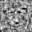
\includegraphics[width=1\linewidth]{full_set.png}
  \caption{full training set thetas}
  \label{fig:a0}
\end{subfigure}%

\begin{subfigure}{.35\textwidth}
  \centering
  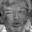
\includegraphics[width=1\linewidth]{each2_set.png}
  \caption{partial training set thetas}
  \label{fig:b0}
\end{subfigure}%
\end{figure*}

We can observe that the thetas get from partial training set which only contains 2 pictures from each person has a clearer face on it. This demonstrates overfit. If we use full training set to get thetas, it will generalize all data so it will look less likely to see a face.
\clearpage
\noindent \textit{(b)Visualizing theta with different max iterations given full training set}

\begin{figure*}[!ht]
\begin{subfigure}{.35\textwidth}
  \centering
  
\includegraphics[width=1\linewidth]{part4ba.png}
  \caption{Figure1:max iterations=30000}
  \label{fig:a1}
\end{subfigure}%

\begin{subfigure}{.35\textwidth}
  \centering
  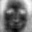
\includegraphics[width=1\linewidth]{part4bb.png}
  \caption{Figure2:max iterations=10}
  \label{fig:b1}
\end{subfigure}%
\end{figure*}
I change different max iterations to control how deep will the gradient descend goes. If it stops early result in Figure2 which looks like a face. With more iterations, the gradient descend will go deeper and created a less face-like image like Figure1. So we can conclude that with more iterations the gradient descend will get more accurate and generalized thetas.


%%%%%%%%%%%%%%%%%%%%%%%%%%%%%%%%%%%%%%%%%%%%%%%%%%%%%%%%%%%%%%%%%%%%%%%



\end{homeworkProblem}
\clearpage

\begin{homeworkProblem}
\noindent \textit{Classifying actors as male or female}
\\
The actors I built classifier on is:
\begin{verbatim}
    act = ['Lorraine Bracco', 'Peri Gilpin', 'Angie Harmon', 
    'Alec Baldwin', 'Bill Hader', 'Steve Carell']
\end{verbatim}
And the final performance test is from these actors:
\begin{verbatim}
    other_act = ['Daniel Radcliffe', 'Gerard Butler', 'Michael Vartan', 
    'Kristin Chenoweth', 'Fran Drescher','America Ferrera']
\end{verbatim}
Following the final result:
\begin{verbatim}
    performance on this 6 actors: 0.890476190476
    performance on other 6 actors:  0.640476190476
\end{verbatim}
We can see that the performance on this 6 actors which built this classifier is much higher than the performance tested on other 6 actors. This demonstrate an over fitting which is because this classifier is optimized and generalized and best matches this 6 actors. However it is to well designed that if it test gender recognition on other people, it will perform worse.
\clearpage
\noindent \textit{Performance on training set and validating set of actors in \textbf{act} versus classifiers built from different sizes of training set}
\begin{figure*}[!ht]
\begin{subfigure}{.35\textwidth}
  \centering
  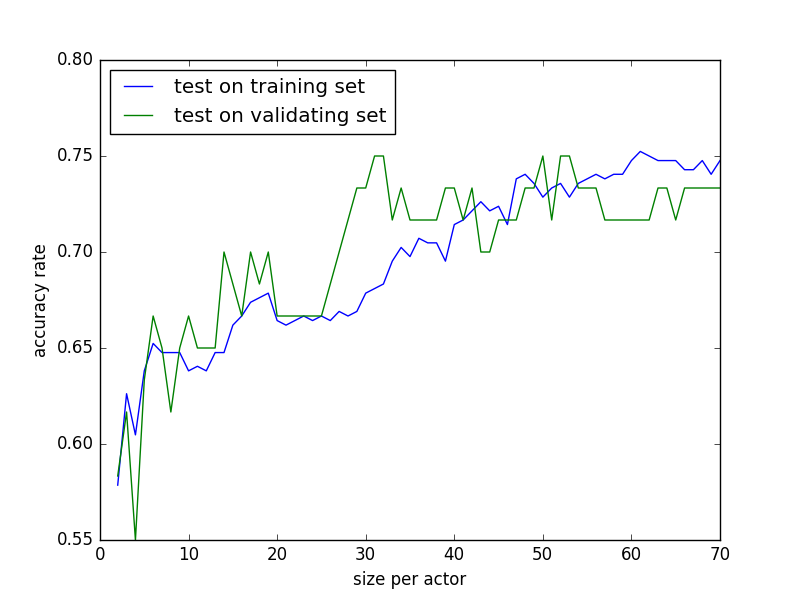
\includegraphics[width=2\linewidth]{part5.png}
  \caption{Figure1:performance vs. set size per person}
  \label{fig:pvs}
\end{subfigure}%
\end{figure*}
\\
We can observe that the performance on training set is increasing as the training set size is increasing, however, as for validating set, after reaching 70\% it starts to fluctuated and won't increase anymore. Indeed, increasing training size will result in increase in accuracy rate, however, the effect will not that great due to overfitting. The difference between after 40 pictures per person is because the thetas are so well fitted into training set itself but it performs unchanged for validating set.
\clearpage
\end{homeworkProblem}

\begin{homeworkProblem}
\noindent \textit{(a)compute gradient}
\begin{figure*}[!ht]
\begin{subfigure}{.35\textwidth}
  \centering
  \includegraphics[width=2\linewidth]{IMG_5280.jpg}
  \caption{Figure1:compute gradient}
  \label{fig:pvs}
\end{subfigure}%
\end{figure*}
\clearpage
\noindent \textit{(b)proof}
\begin{figure*}[!ht]
\begin{subfigure}{.35\textwidth}
  \centering
  \includegraphics[width=2\linewidth]{IMG_5282.jpg}
  \caption{Figure1:proof}
  \label{fig:pvs}
\end{subfigure}%
\end{figure*}
\clearpage
\noindent \textit{(c)code for cost function and gradient}
\\
Code I use to compute cost:
\begin{verbatim}
    def multi_f(x, y, theta):
        x = vstack((ones((1, x.shape[1])), x))
        return sum(sum((dot(theta.T, x) - y) ** 2))
\end{verbatim}
Code I use to compute gradient:
\begin{verbatim}
    def multi_df(x, y, theta):
        x = vstack((ones((1, x.shape[1])), x))
        return 2 * dot(x, (dot(theta.T, x) - y).T)
\end{verbatim}
Suppose I have N pictures and M labels,
here I use x which is the flatten picture stacks with shape (1025,N),each column represents a picture, y which is the target labels with shape (M,N), theta with shape (1025,M)
\clearpage
\end{homeworkProblem}
\clearpage
\noindent \textit{(d)experimenting h}
\\
Code I use to get finite differences and compare to the gradient function we produce is:
\begin{verbatim}
    def finite_difference(x, y, theta, h):
        origin_t = multi_f(x, y, theta)
        theta = theta + np.full((theta.shape[0], theta.shape[1]), h)
        after_t = multi_f(x, y, theta)
        finite_diff = (after_t - origin_t)/h
        total_error = sum(finite_diff - multi_f(x, y, theta))
        return abs(total_error)/(1025*6*1.0)
\end{verbatim}
I first get an original cost function and then add \textbf{h} to every theta array's entry to produce a cost function with augmented theta. I subtract them and divide it by h to get the finite difference. Then I use finite difference to subtract the derivative we get from our gradient function \textbf{multi\_df} and calculate the average error.
\begin{figure*}[!ht]
\begin{subfigure}{.35\textwidth}
  \centering
  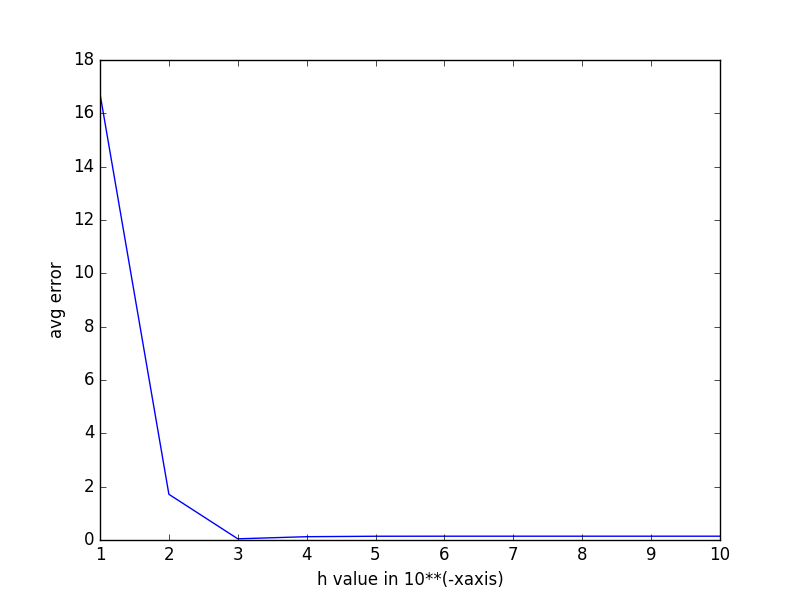
\includegraphics[width=2\linewidth]{part7.png}
  \caption{Figure1:average error vs. h}
  \label{fig:pvs}
\end{subfigure}%
\end{figure*}
\\
We can observe that with a rather small h, the average error is far smaller than a big h, but not too small or else it will cause a slightly more error. It also suggests that our gradient function is correct.
\clearpage
\begin{homeworkProblem}
The gradient descend will perform on following actors:
\begin{verbatim}
    act = ['Lorraine Bracco', 'Peri Gilpin', 'Angie Harmon', 
    'Alec Baldwin', 'Bill Hader', 'Steve Carell']
\end{verbatim}
And I labeled them:
\begin{verbatim}
    act_labels = {'bracco': [1, 0, 0, 0, 0, 0], 
                  'gilpin': [0, 1, 0, 0, 0, 0], 
                  'harmon': [0, 0, 1, 0, 0, 0],
                  'baldwin': [0, 0, 0, 1, 0, 0], 
                  'hader': [0, 0, 0, 0, 1, 0], 
                  'carell': [0, 0, 0, 0, 0, 1]}
\end{verbatim}
First I tested the right alpha, still, I picked a fairly large max iteration
\\
\begin{figure*}[!ht]
\begin{subfigure}{.35\textwidth}
  \centering
  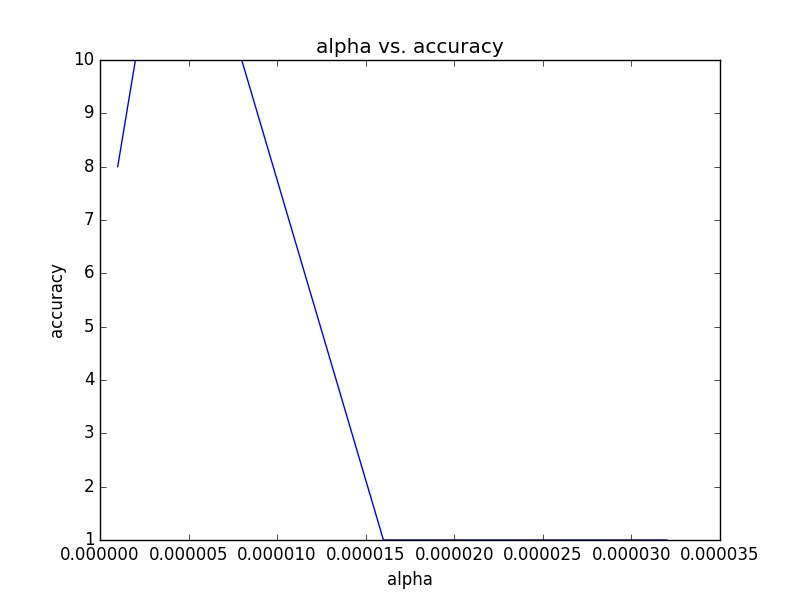
\includegraphics[width=1\linewidth]{testalphap7.png}
  \caption{Figure1:max iterations fixed to 30000}
  \label{fig:a1}
\end{subfigure}%
\end{figure*}
\\
The graph shows some similarity with the previous alpha vs. accuracy graph in part3 and the alpha selection is alright for this question too.
So I choose the same alpha and max iteration as before.
\\
Code I use to compute the output and accuracy:
\begin{verbatim}
result_t = 0
for name, files in names_set.items():
    if name in act_nickname:
        for i in files[:70]:
            pic1 = imread('cropped/' + i).flatten() / 255.
            pic1 = np.insert(pic1, 0, 1)
            pic1 = pic1.T
            result1 = dot(theta.T, pic1)
            if np.argmax(result1) == act_labels[name].index(1):
                result_t += 1
accuracy=result_t/420.
\end{verbatim}
Code I use to get predicted label is:
\begin{verbatim}
    result = dot(theta.T, pic1)
\end{verbatim}
Suppose result for baldwin may look like [0.367739812 0.452342234 0.56352423 0.234134134 0.87981623 0.412423412]
\\
Here I use \textbf{np.argmax(result1) ==act\_labels[name].index(1)} to compare the prediction and the target.
What it does is get the maximum number's index in the prediction and to see if it matches the number 1's index in its label.
In this case, baldwin's label is [0, 0, 0, 1, 0, 0] and its 1's index is 3 and the maximum number's index in the prediction is 4, thus this picture is not a correct guess.
\\
\noindent \textit{The result:}
\begin{verbatim}
    accuracy for training_set:  0.847619047619
    accuracy for validation set:  0.516666666667
\end{verbatim}
We can observe that there's a decreasing in accuracy compared to just distinguish one person from others. This is because the thetas are more look like a face and thus more optimized for the training set. This will cause a not so generalized theta and decrease in accuracy in validation.
\end{homeworkProblem}
\clearpage


\begin{homeworkProblem}
\noindent \textit{Visualizing thetas}
\\
The theta pictures are generated using scipy.misc.imsave so the theta image appear to be gray.


\begin{figure*}[!ht]
\begin{subfigure}{.35\textwidth}
  \centering
  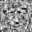
\includegraphics[width=0.35\linewidth]{baldwin.png}
  \caption{baldwin thetas}
  \label{fig:a0}
\end{subfigure}%

\begin{subfigure}{.35\textwidth}
  \centering
  
\includegraphics[width=0.35\linewidth]{gilpin.png}
  \caption{gilpin thetas}
  \label{fig:b0}
\end{subfigure}%

\begin{subfigure}{.35\textwidth}
  \centering
  
\includegraphics[width=0.35\linewidth]{hader.png}
  \caption{hader thetas}
  \label{fig:a0}
\end{subfigure}%

\begin{subfigure}{.35\textwidth}
  \centering
  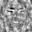
\includegraphics[width=0.35\linewidth]{bracco.png}
  \caption{bracco thetas}
  \label{fig:b0}
\end{subfigure}%

\begin{subfigure}{.35\textwidth}
  \centering
  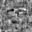
\includegraphics[width=0.35\linewidth]{carell.png}
  \caption{carell thetas}
  \label{fig:a0}
\end{subfigure}%

\begin{subfigure}{.35\textwidth}
  \centering
  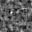
\includegraphics[width=0.35\linewidth]{harmon.png}
  \caption{harmon thetas}
  \label{fig:b0}
\end{subfigure}%
\end{figure*}
The algorithm works and produces 6 thetas for each person. The thetas have some resemblance with the actors which is perfectly fine because the prediction is basically \textbf{dot(theta.T,picture)}, with a clearer face, the dot product is bigger at the same index its label has 1.


\clearpage

\end{homeworkProblem}
\clearpage

%----------------------------------------------------------------------------------------

\end{document}